\chapter{The Partially Synchronous Model, 33\%, and the CAP Principle}
\section{Overview}
This chapter has three goals. The first is to introduce you to the “partially synchronous”
model of computation, which interpolates between the synchronous model (studied in chapters 2 and 3) and the asynchronous model (the subject of chapters 4 and 5). If you
remember only one model of message delivery, this should probably be the one. It’s a “sweet
spot” model in that its assumptions are weak enough to make it relevant to the design of
Internet-scale distributed protocols, but also strong enough so that interesting protocols with
provable guarantees exist.\\
The second goal is to establish limitations on what we can hope for in the partially
synchronous model. In particular, we’ll prove an impossibility result that rules out strong
positive results in the case that at least one-third of the nodes can be Byzantine (i.e., $f \geq \frac{n}{3}$,
where n is the number of nodes and $f$ is an upper bound on the number of Byzantine nodes).
Whenever you hear about a critical “33\%” threshold in a blockchain whitepaper or technical
discussion, it boils down to this impossibility result. As a bonus, the proof is not too bad
(certainly easier than the proof of the FLP impossibility result) and the basic intuition
behind is something that you can retain for a long time to come.\\
The third goal of this chapter is to discuss a famous principle from distributed systems,
the “CAP Principle.” The letters stand for “consistency,” “availability,” and “partition tolerance,” and the principle states that you must pick two of these three properties (you can’t
have them all). The CAP principle superficially resembles the FLP impossibility theorem
for the asynchronous model, and it’s important to understand the differences between them.
After this chapter, when you hear someone appeal to the CAP principle to justify their
system’s weaknesses, you’ll be in a position to assess whether they know what they’re talking
about.\\

\section{The Story So Far}
To set the stage for the partially synchronous model, let’s review the two models of communication that we’ve studied thus far (in chapters 2 and 3 and chapters 4 and 5, respectively):
\nt{
\begin{center}
    \textbf{Recap: Synchronous vs. Asynchronous Model}
\end{center}

\noindent
\textbf{Synchronous model:}
\begin{itemize}
    \item shared global clock;
    \item a priori known bound $\Delta$ on the maximum message delay;
    \item good news: strong positive results possible (e.g., from chapter 2, with
    the PKI assumption, the Dolev-Strong protocol, and the consequent SMR
    protocol that can tolerate 99\% Byzantine nodes);
    \item bad news: overly strong assumption (rules out network outages and attacks of unexpected durations)
\end{itemize}
\noindent
\textbf{Asynchronous model:}
\begin{itemize}
    \item no global clock;
    \item no assumptions on message delays other than that every message eventually gets delivered;
    \item good news: with such weak assumptions, any positive result (i.e., consensus protocol with provable guarantees) is automatically interesting and
    impressive;
    \item bad news: by the FLP impossibility theorem, no deterministic protocol
    can solve Byzantine agreement (or state machine replication) with the
    threat of even a single crash fault.
\end{itemize}
}
\noindent
\textbf{Synchronous model.} In the synchronous model, there’s a shared global clock: all nodes
agree at all times on the current time step (with no communication needed). There’s
also an assumed bound $\Delta$ on the maximum number of time steps that a message might get
delayed (any message sent in a time step $t$ is guaranteed to arrive by time step $t + \Delta$, if not
earlier). The value of the parameter $\Delta$ is known upfront, meaning that the description of a
protocol can depend on it.\\
We saw in Chapter 2 that strong positive results are possible in the synchronous model (at
least under the PKI assumption), with the Dolev-Strong protocol for Byzantine broadcast
resilient to even 99\% of the nodes being Byzantine. Using our standard rotating leaders trick,
leads to an equally fault-tolerant protocol for the (multi-shot) state machine replication
(SMR) problem.\\
On the other hand, while the shared global clock assumption is perhaps somewhat palatable, the known bound on worst-case message delay is an unreasonable assumption for protocols that operate at the scale of the Internet. The Internet does suffer long outages
on occasion, and blockchain protocols that secure billions of dollars of value will inevitably
have to deal with long-lasting attacks.\\

\noindent
\textbf{The asynchronous model.} The asynchronous model is the polar opposite of the synchronous
model, with no global shared clock and no guarantees whatsoever about message delivery
(other than the minimal assumption that every message eventually gets delivered, after
some finite delay). Because this model’s assumptions are so weak (requiring only a barely
functioning communication network), any protocol with strong provable guarantees would
automatically be interesting. Unfortunately, the FLP impossibility theorem showed us that
this model throws out the baby with the bathwater, in the sense that no good consensus
protocols exist (without resorting to randomization or extra timing assumptions), even under
the threat of a single Byzantine (or even crash fault) node.\\
The synchronous and asynchronous models are probably the two most natural models of
communication to write down. But neither model guided us toward what we want: a
consensus protocol that might plausibly be useful at the Internet scale. It’s thus clear that
we need a third model that interpolates between the synchronous and asynchronous
models, with assumptions weak enough to be relevant to Internet-scale protocols but strong
enough such that useful consensus protocols with provable guarantees exist. Such a model
is the subject of this chapter.

\section{The Partially Synchronous Model}
\subsection{Intuition: Recovery After an Attack/Outage Eventually Ends}

We rejected the synchronous model on the grounds that network outages and attacks of
unexpected durations will at some point occur. But outages and attacks must end eventually,
right? Maybe it takes a few hours, or maybe a few days, but surely we’re interested in a
world where at some point the world becomes “normal” again.\\
A key idea in the partially synchronous model is to explicitly declare some periods of
time “normal” (and thus well-modeled by the synchronous model) and other periods “under
attack” (and thus appropriately modeled by the asynchronous model). The goals then would
be:
\begin{itemize}
    \item (sanity check) achieve everything you want (e.g., safety and liveness) during “normal
operation conditions”; 
    \item (stress test) don’t break too badly when under attack (e.g., give up only safety, or only
liveness); We will be identifying an attack phase with the asynchronous model that we discussed in the last two chapters. The FLP impossibility result says that if we're in an asynchronous phase and we're under attack during that time we cannot have everything that we want, we cannot have
both safety and liveness but we'd still like to aspire to giving up as little as possible while we're under attack so at
least we keep safety or at least we keep aliveness.
    \item (recovery) recover quickly after an attack once the network returns to normal operating
conditions. After an attack ends and after we switch from asynchrony to a synchronous setting, we would like to then have the guarantees we expect in the synchronous setting for example safety and liveness.
\end{itemize}

One could imagine a model in which there’s an arbitrary number of alternative synchronous and asynchronous phases. We’ll work with the most minimal version of this idea
in which there’s a single synchronous phase and a single asynchronous phase. (Chaining
together several copies of the minimal model essentially recover the case of an arbitrary
number of alternations.) To study recovery after an attack (the third goal above), it makes
sense to have the asynchronous phase first, followed by the synchronous phase.
\subsection{The Formal Definition}
Next is (one of) the formal definition of the partially synchronous model. This definition is
due to Dwork, Lynch, and Stockmayer; the same authors proved some fundamental
possibilities and impossibility results in the same paper.\\

\noindent
\textbf{Timing assumptions.} The first assumption is that, like in the synchronous model, there
is a shared global clock. That is, whether under attack or in normal operating conditions, all
nodes automatically agree (without any communication) on what the current time step is.
While we’d rather not have this assumption, it’s definitely the more palatable of
the two assumptions that we made in the synchronous model (and you can start imagining
ways of approximating it in practice).\\

\noindent
\textbf{The synchronous phase.} Second, there will be a parameter $\Delta$ that specifies the maximum delay (in time steps) that a message might suffer in the synchronous phase. During the
initial asynchronous phase, the parameter $\Delta$ plays no role. Like in the synchronous model,
in (this version of) the partially synchronous model, we assume that the value of $\Delta$ is known
up front and that the protocol description can depend on it. For example, you could think of
each time step as representing one millisecond and $\Delta$ equal to 1000 or 2000 (1 or 2 seconds).\\

\noindent
\textbf{GST: the transition point.} Finally, there is a parameter that dictates when the underlying communication network switches from synchronous to asynchronous mode, called
the global stabilization time or the GST. Unlike the parameter $\Delta$, the parameter GST is not
known upfront and so a protocol description cannot depend on it. In other words, a protocol
is responsible for providing its guarantees no matter what the GST might be. A protocol is not informed when the GST occurs, so it effectively must detect its passing automatically
(and resume normal operation accordingly). Therefore, it's very important that the global stabilization time is unknown to the protocol; the protocol should work
simultaneously for all possible GSTs.
Taken together, the parameters GST and $\Delta$ impose the following constraints on message
delivery (for the a priori known parameter $\Delta$ and whatever value of the GST the message
delivery adversary happens to choose):
\begin{enumerate}
    \item (messages sent in asynchronous phase) if a message is sent at time step $t$ with $t \leq GST$,
then it is received by the intended recipient at or before time step $GST + \Delta$ (i.e., as if
it was sent at time GST);
    \item (messages sent in synchronous phase) if a message is sent at time step $t$ with $t \geq GST$,
then it is received by the intended recipient at or before time step $t + \Delta$.
\end{enumerate}

Because the GST must be finite, every message that is sent must eventually be delivered.
In this sense, the partially synchronous model is a special case of the asynchronous model.
The asynchronous model is strictly more general, as message delivery there does not need
to obey any quantitative constraints such as the ones above.
The value of the GST must be unknown to the protocol. In effect, the adversary
controls message delivery and chooses it as a function of the chosen protocol. One reason
is conceptual: the whole point of the partially synchronous model is to force us to reckon with
network outages and attacks of unexpectedly long duration. Another reason is technical:
were the GST known upfront, all possibility results for the synchronous model (e.g., the
Dolev-Protocol) would port over immediately with a stalling pre-processing step (the protocol
could simply wait until the GST and then proceed as in the synchronous model).\\

\noindent
\textbf{Protocols.} We’ll later prove an impossibility result for the partially synchronous
model, and for that, we’ll need a precise definition of what a protocol can and cannot do. In
the asynchronous model, a protocol defined the action of a node (i.e., which messages to send)
as a function of what the node knows, namely its private input and the sequence of messages
it has received thus far. Because the partially synchronous model introduces some timing
assumptions, nodes have additional information: the current time step and the precise
time step at which each received message arrived. A protocol is then defined as a function
from the node’s current knowledge (private input, current time step, messages received, and
their arrival times) to an action (which messages to send out and to whom). Unlike in the
asynchronous model, protocols in the partially synchronous model can implement timeouts
(e.g., ignoring messages that arrive many time steps after they were expected). Next chapter
we’ll see how the Tendermint protocol takes advantage of this additional power.\\

\noindent
\textbf{The “unknown $\Delta$” model.} Somewhat confusingly, there are two conceptually distinct
versions of the partially synchronous model (both defined by Dwork, Lynch, and Stockmeyer). Throughout this chapter series, we’ll focus on the “GST” version of the partially
synchronous model that we've been discussing thus far. Elsewhere, you might also encounter
a second version of the model, so let’s discuss that briefly next.\\
The second version of the model connects strongly to our discussion at the beginning of
chapter 4. There, we made a naive attempt at relaxing the synchronous model (with $\Delta$ = 1)
to a model with variable message delays (anywhere from 1 up to a known upper bound $\Delta$).
We then noticed that any possibility result for the $\Delta = 1$ model extends automatically to
the general (but known) $\Delta$ case through “time inflation,” with all nodes always waiting $\Delta$
time steps in between consecutive actions to make sure all messages sent by honest nodes are
received in time. Dissatisfied, we pined for a consensus protocol whose speed is not dictated
by the worst-possible message delay, and rather adapts automatically to the network speed
and is fast whenever the underlying communication network is fast. This is exactly the idea
behind the second version of the partially synchronous model.\\
In the “unknown $\Delta$” version of the model, there’s no GST, and no transition between an
asynchronous and a synchronous phase. Messages will literally always get delivered within
$\Delta$ time steps, just like in the synchronous model. Unlike the synchronous model (and the
“GST version” of the partially synchronous model, however, the parameter $\Delta$ is not known
in advance and the protocol description cannot depend on it. In other words, a protocol
must work simultaneously in every instantiation of the synchronous model (i.e., whatever
the network speed/parameter $\Delta$).

\noindent
\textbf{Why two versions?} The two versions of the partially synchronous model both seem
natural—the “GST version” encodes the goal of quick recovery after an outage or attack,
and the “unknown $\Delta$” version the goal of operating at network speed (whatever that may
be)—but also rather different. Why do they go under the same name? One reason is that the
original paper introduced both versions under the umbrella of “partial synchrony.” This
tradition has persisted to the present day largely because possibility and impossibility results
that hold in one of the two versions tend to hold also in the other version. The two versions are thus roughly (but not formally) equivalent
for our purposes. It’s a good exercise to rework the proof of Theorem 6.5.1 (stated for the
“GST version”) so that the same impossibility result holds for the “unknown $\Delta$” version of
the partially synchronous model. Similarly, you might want to think about how to rework
the Tendermint protocol (covered in the forthcoming chapter 7) so that its consistency and
liveness guarantees (with $f < \frac{n}{3}$) hold also in the “unknown $\Delta$” model. We won’t discuss
this version of the model again in these lessons.

\section{Goals for a Consensus Protocol}
In the partially synchronous model, what should we ask for from a consensus protocol? For
example, when should we deem a protocol a “solution” to the Byzantine agreement problem
in the partially synchronous model? As a quick reminder (from chapter 4), in the Byzantine
agreement problem, every node $i$ has a private input $v_i$ (drawn from some set $V$ ) and the
goals are:
\nt{
\begin{center}
    \textbf{Desired Properties of a Byzantine Agreement Protocol}
\end{center}
\begin{enumerate}
    \item \textbf{Termination.} Every honest node i eventually halts with some output $w_i \in V$.
    \item \textbf{Agreement.} All honest nodes halt with the same output (no matter
what the private inputs are).
    \item \textbf{Validity.} If $v_i = v^*$ for every honest node $i$, then $w_i = v^*$ for every honest node $i$.
\end{enumerate}
}

The FLP impossibility result (chapters 4 and 5) tells us that no consensus protocol guarantees all of these properties in the asynchronous model. The partially synchronous model is
less general that the asynchornous model (on account of the constraints on message delivery
spelled out in Section 6.3.2), so the FLP impossibility result does not immediately apply.
It does apply during the asynchronous phase of the partially synchronous model, and so every
protocol that guarantees validity and agreement on termination must in some cases not terminate until after the global stabilization time. In other words, if no violations of validity or
agreement are allowed, a protocol cannot guarantee liveness during the asynchronous phase.
By the same reasoning, for the SMR problem, no protocol that always guarantees consistency
can guarantee liveness prior to the global stabilization time. Post-GST, however, there is
hope of guaranteeing both safety and liveness.\\

Summarizing, the best we could hope for would seem to be:
\begin{itemize}
    \item at least one of the safety or liveness during the asynchronous phase;
    \item safety and liveness during the synchronous phase (beginning not long after the GST).
\end{itemize}
What should we give up during the asynchronous phase? Arguably the most natural choice,
and the only choice explored in 20th-century research on the partially synchronous model,
is to give up liveness and preserve safety. Safety properties state that “something bad never
happens” and it’s sensible to interpret “never” as “including in the asynchronous phase.”
Liveness properties assert “something good eventually happens,” and “eventually” might
naturally be interpreted as “after the GST.”

\nt{
\begin{center}
    \textbf{Traditional Goals in the Partially Synchronous Model}
\end{center}
\begin{enumerate}
    \item Safety: Safety holds always, even in the asynchronous phase.
    \item Eventual liveness: Not long after the GST, safety and liveness both
hold (e.g., consistency and liveness for SMR);
\end{enumerate}

}
Many blockchain consensus protocols adopt these same two goals, and this will be our focus
in this and the next chapter. That said, one interesting aspect of longest-chain consensus (discussed in chapter 8) is that it makes non-traditional compromises in periods of asynchrony, favoring liveness over safety.

\section{The Big Result}
When are safety and eventual liveness achievable in the partially synchronous model for the Byzantine agreement problem? Turns out there’s a remarkably crisp answer to this
question, with the magical threshold being 33\%. (Remember that $n$ always denotes the
number of nodes and $f$ the upper bound on the maximum number of Byzantine nodes.)
\thm{}{ There exists a deterministic protocol for the Byzantine agreement problem that satisfies agreement, validity, and eventual (post-GST) liveness in the partially synchronous model if and only if $f < \frac{n}{3}$.}
This is two results in one, a possibility result and a matching impossibility result.
We’ll take up the impossibility result—that with $f \geq \frac{n}{3}$, no Byzantine agreement protocol
can achieve safety and eventual liveness. In chapter 7 we’ll study the Tendermint protocol,
which does in fact achieve safety and eventual liveness provided $f < \frac{n}{3}$. Some comments:
\begin{enumerate}
    \item Tendermint is only one protocol among many that achieves optimal fault tolerance in
the partially synchronous model. (For example, the original paper also describes a
solution.) Tendermint is an obvious one for us to single out, as it is used in several major blockchain protocols.
    \item Theorem 6.5.1 holds whether or not we make a PKI assumption. The impossibility
result we’ll prove in this chapter holds even under the PKI assumption (Byzantine
nodes won’t need to forge any signatures to carry out their devious strategy). The
Tendermint protocol makes use of a PKI assumption, but the same positive result is
possible (with a different protocol) without it.
    \item Like the FLP impossibility theorem from chapters 4 and 5, this impossibility result
is stated for the Byzantine agreement problem but applies equally well to the SMR problem.6 The Tendermint protocol in chapter 7 solves the SMR problem, which can
in turn be used to construct (via the reduction in footnote 6) an equally fault-tolerant
Byzantine agreement protocol.
    \item You frequently see distributing computing experts write the f < n/3 assumption as,
equivalently, $n \geq 3f + 1$. This is a famous, almost meme-like inequality in distributed
computing—if no conference has yet printed T-shirts with “$n \geq 3f + 1$” on the front,
it’s long overdue!
    \item Whenever you hear a blockchain person or whitepaper refers to a “33\% threshold”—
generally to justify why a protocol isn’t more robust to attacks than it already is, it
boils down to the one in Theorem 6.5.1.
    \item If you remember only one result from this boot camp on permissioned consensus (chapters 2–7), Theorem 6.5.1 would be a good one. It is the culmination of our study of the 20th-century literature on the design and analysis of consensus protocols.
\end{enumerate}

\section{Intuition for Impossibility}
The goal of this section is to provide you with reasonably accurate intuition about why
the “only if” direction of Theorem 6.5.1, the impossibility result, is true. This intuitive
argument should demystify where the magical “33\% comes” from, which in hindsight should
seem preordained. The informal argument is compact enough that you should be able to
remember it for a significant period of time. Because the result is so important, I must also offer you full proof of this, see Section 6.7.
The role of unbounded message delays. First, let’s talk about the proof strategy and the
ingredients we expect to see in the argument. Theorem 6.5.1 is not the first “33\%” impossibility
result that we've seen. The PSL-FLM result from Chapter 3 established the same
threshold for the Byzantine broadcast problem in the synchronous model when there is no
PKI assumption. Are these the same “33\%”? Perhaps Theorem 6.5.1 can somehow be reduced
to the PSL-FLM result that we worked so hard to prove in Chapter 3? Maybe there’s no
real difference as to the degree of fault tolerance possible in the synchronous and partially
synchronous models?\\
In fact, completely different forces are driving the two impossibility results. Remember
that the PSL-FLM impossibility result does not hold with the PKI assumption, 
the Dolev-Strong protocol (chapter 2) solves the Byzantine broadcast problem (i.e., satisfies
agreement, validity, and termination) in the synchronous model even when 99\% of the nodes
are Byzantine. As a consequence, its proof must crucially hinge on the lack of PKI. This dependence showed up in a subtle way, the proof uses clever strategies for Byzantine nodes
that involve the simulation of four honest nodes (in the “hexagon thought experiment”), and these strategies are infeasible under the PKI assumption (because it
would require forging signatures without knowledge of the appropriate private key, which
with PKI we assume is impossible).
As mentioned in the previous section, Theorem 6.5.1 is true whether or not we make the
PKI assumption. Presumably, then, the proof of Theorem 6.5.1 in Section 8 will not by making
use of strategies for Byzantine nodes that involve the simulation of honest nodes. This was
the only trick used in the proof of the PSL-FLM impossibility result, so something else must
be driving the “33\%” in Theorem 6.5.1. Given that the result is for the partially synchronous
(as opposed to synchronous) model, presumably the proof will be driven by the threat of
potentially unbounded message delays.\\

\noindent
\textbf{Intuition, part 1:} plausibly deniable silent treatment. First, even in the synchronous
model, in order to satisfy termination, an honest node must be prepared to halt with an
output even if it hasn't heard anything at all from some of the other nodes. After all, one
strategy for the Byznatine nodes is to give the honest nodes the silent treatment and never
send out any messages. Because up to $f$ nodes may be Byzantine, an honest node can only
count on hearing from $n − f$ nodes (counting itself) before needing to make a decision.\\

\noindent
\textbf{Intuition, part 2: wolves in sheep’s clothing.}
Because we’re now in the partially
synchronous model, there’s an equally plausible explanation for why an honest node might
not have ever heard from a set of other nodes, maybe those nodes are actually honest and
sent all the messages that they were supposed to send, but all of their messages have been
delayed for a very long time. (This is only possible before the global stabilization time, but
remember that the GST is unknown to the protocol can be arbitrarily large.) This cannot
happen in the synchronous model. If you don’t hear the messages that you expect coming
in from some node, the only possible explanation is that that node is Byzantine.
Thus, the real bummer is that when an honest nodes takes action after hearing from only
$n − f$ nodes (as it must), for all it knows $f$ of the voices its hearing belong to Byzantine nodes
(with all the as yet unheard from nodes honest but suffering massively delayed messages).
Like wolves in sheep’s clothing, these Byzantine node might lead the honest node astray
by feeding it bad information (e.g., pretending their private input was 1 rather than 0).
Intuitively, if at least 50\% of these $n − f$ nodes are Byzantine, there’s no way for the honest
node to determine whom to believe. (If a strict majority of them are honest, one might hope
that some kind of majority vote could indicate the appropriate action.) This leads to the
requirement that $f < \frac{1}{2}(n − f)$ or, equivalently, that $f < \frac{n}{3}$.

\nt{
\begin{center}
    \textbf{Demystifying the 33\%}
\end{center}
\begin{enumerate}
    \item An honest node can only wait to hear from $n − f$ nodes (counting itself)
before taking action. By the termination requirement and the fact that Byzantine nodes may never respond.
    \item To avoid getting tricked, a strict majority of these $n − f$ nodes must be honest (and so $f < \frac{1}{2}(n − f)$ or $f < \frac{n}{3}$). The $f$ as-yet-unheard-from nodes may be honest (with their messages massively delayed), meaning $f$ of the $n − f$ nodes that have been heard from may yet be Byzantine.
\end{enumerate}
}
This informal argument highlights the challenge of de facto collusion between the Byzantine
nodes and adversarial message delivery. Both Byzantine nodes and the adversary controlling
message delivery have to the power to enforce silence from $f$ nodes for an arbitrarily long
period of time, and an honest node cannot distinguish whom is the culprit. In effect, each
Byzantine node winds up knocking out two honest nodes, one honest node whose contributions are ignored (because they are massively delayed and it gets mistaken for a Byzantine node) and a second honest node whose received messages are cancelled by conflicting messages sent by a Byzantine node. Intuitively, we need one honest node still standing after all these knockouts, meaning $(n − f) − 2f > 0$ or, equivalently, $f < n/3$.
All this is accurate and hopefully retainable intuition about why (the “only if” direction
of) Theorem 6.5.1 is true, but none of it constitutes an actual convincing proof. So let’s get
to it!
\section{Proof of Theorem 6.5.1 (“Only If” Direction)}
\noindent
\textbf{Statement of impossibility result:} Recall what we’re trying to prove: in the partially
synchronous model (defined in Section 6.3.2), with or without the PKI assumption, for every
$f$ and $n$ with $f \geq \frac{n}{3}$, no Byzantine agreement protocol achieves the goals spelled out in
Section 6.4: agreement (always), validity (always), and termination (eventually, possibly only
after the GST).\\

\noindent
\textbf{A simple case capturing all the complecxity.} We’re going to focus on the simplest possible case of the impossibility result, with $n = 3$ and $f = 1$ (three nodes, one of which
might be Byzantine). (We did the same thing back in chapter 3 for the PSL-FLM impossibility result for Byzantine broadcast in the synchronous model without the PKI assumption.)
Your first reaction might be that this assumption trivializes the result, but the truth is the
exact opposite—this special case already captures all of the complexity and nuance of the
general impossibility result. A good exercise is to rework the following argument so that it
applies to your favorite choice of $n$ and $f \geq \frac{n}{3}$.
Call the three nodes “Alice (A),” “Bob (B),” and “Carol (C)” and see Figure 6.1. Toward
a contradiction. Suppose there is a Byzantine agreement protocol $\pi$ that satisfies agreement
(always), validity (always), and termination (eventually). Consider the scenario in which
Alice is honest and has a private input of 1, Carol is honest and has a private input of 0,
and Bob is Byzantine (and hence his private input doesn't matter).\\

\begin{figure}[h]
    \centering
    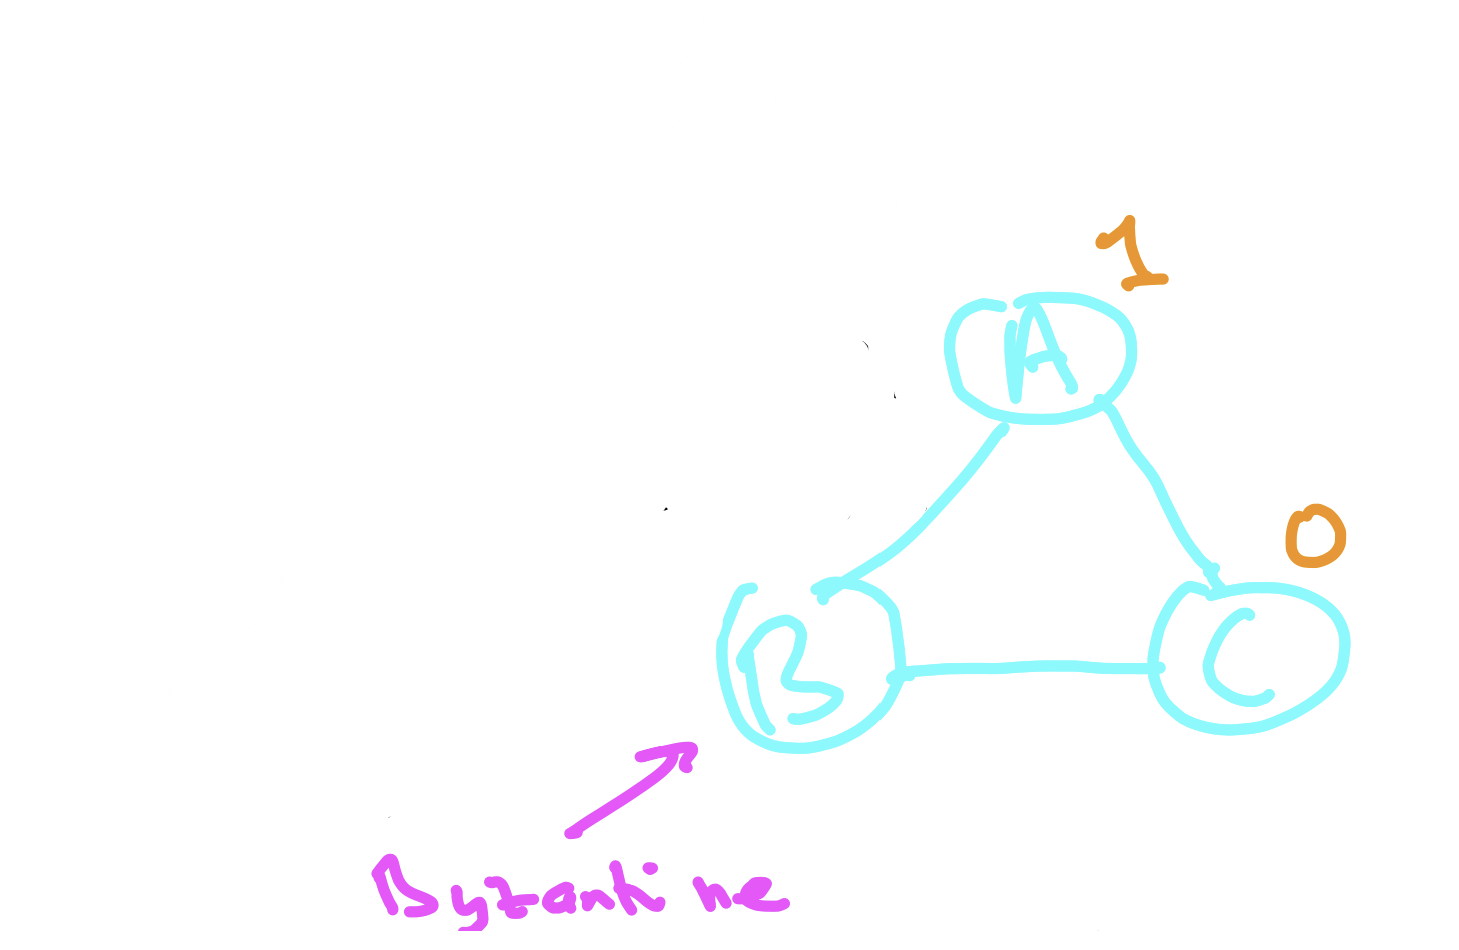
\includegraphics[scale = 0.5]{figures/f20.png}
    \caption{Proof of impossibility:$f \geq \frac{n}{3}$}
    \label{fig:mesh1}
\end{figure}\\

\noindent
\textbf{The adversaries’ collusive strategy.} Imagine that Bob engages in the canonical Byzantine ploy of sending inconsistent messages to different honest nodes, while aided and abetted by the adversary controlling message delivery. Specifically:
\begin{itemize}
    \item The adversary controlling message delivery delays all messages between Alice and Carol
for a long time. (How long? See below.)
    \item Bob interacts with Alice as if he has a private input of 1 and never received any
messages from Carol.
    \item Bob interacts with Carol as if he has a private input of 0 and never received any
messages from Alice.
\end{itemize}

Note that Bob is perfectly capable of carrying out this strategy (whether or not we’re working
with the PKI assumption). All he has to do is run (two copies of) $\pi$ with the above fabricated
private inputs and message sequences. Because the GST in the partially synchronous model
can be arbitrarily large (as a function of the specific protocol $\pi$), the adversary controlling
message delivery has the power to delay messages between Alice and Carol for as long as it
wants (as they as they are eventually delivered).
Two catch-22s. Now adopt Alice’s perspective, being fed a constant stream of (mis)information
from Bob and silence from Carol. Alice is perfectly aware of the possibility of the scenario
above, that Bob is Byzantine and using the above strategy when Carol’s honestly sent messages are stuck in a pre-GST limbo. Unfortunately, there’s an equally plausible explanation
for what Alice is seeing: perhaps Bob is honest and really does a private input of 1, while
Carol is the Byzantine one and is providing both Alice and Bob with the silent treatment. To hedge
against the latter scenario, because $\pi$ satisfies eventual termination (by assumption), Alice
must eventually (by some finite time $T_1$, and with no input from Carol) output her answer.
By validity (since in the second scenario both honest nodes have the same private input),
her output must be 1.
Carol finds herself in her own catch-22 situation. She’s well aware that reality might
be the first scenario, with Bob the Byzantine one and Alice’s honestly sent messages stuck
in pre-GST limbo. But an equally plausible explanation for what she’s seeing is that Bob
really is honest with a private input of 0, with Alice the Byzantine one who is providing both
Bob and Carol the silent treatment. Because of the threat of the latter scenario, Carol has
no choice but to output her answer by some finite time $T_2$ (with no input from Alice). By
validity, because in that scenario, she and (the other honest node) Bob both have a private
input of 0, her output must be 0.\\

\noindent
\textbf{Putting it all together.} To complete the description of the collusion between the Byzantine node and the adversarial message delivery, assume that all messages between Alice and
Carol are delayed for $\text{max}\{T_1, T_2\} + 1$ time steps (which is allowed provided the adversary
chooses the GST to be at least this large). With Bob behaving inconsistently as above, and
with all communication between Alice and Carol severed Alice outputs 1 (unable to rule out the case in which Bob is honest and Carol gives her the silent treatment), and Carol outputs 0 (unable to rule out an honest Bob and a silent Alice). But Alice and Carol are both
honest nodes, so this outcome of the protocol contradicts the assumption that the protocol $\pi$
satisfies agreement. We can conclude that no such protocol $\pi$ exists, completing the proof
of the “only if” direction of Theorem 6.5.1.

\section{The CAP Principle}
\subsection{The Principle and Its Interpretations}
The CAP Principle is a well-known observation in distributed systems. You might think
that “CAP” indicates the first letters of three last names (as with PSL, FLM, or FLP!), but
the letters actually stand for three informal properties that you would want a distributed
system to satisfy. To interpret them, you might want to think about our running 20th century example in which a big company like IBM is replicating a database to achieve higher uptime.
\begin{enumerate}
    \item ‘C’ stands for “consistency.” It plays a similar role that consistency has played in our
study of the SMR problem. In our running example, consistency would mean that
the answer to a database query should not depend on which replica it gets routed to.
More generally, you would like the experience of a user of a distributed system to be
indistinguishable from interacting with a centralized system (like a single database on
a single server).
    \item ‘A’ stands for “availability,” which resembles the liveness property that we required for
SMR protocols. In our running example, if a user of the database inserts a new entry,
that change should eventually be reflected in future queries to the database. More
generally, any command that a client issues to a distributed system should eventually
be carried out.
    \item ‘P’ stands for “partition tolerance.” Here a partition means a long-lasting severance
of all communication between two different groups of nodes (Figure 6.2). For instance, 
due to a long denial-of-service attack. Partition-tolerance informally means that you’d
like consistency and availability to hold even in the presence of a network partition,
and bears some resemblance to the asynchronous phase of the partially synchronous model
defined in Section 6.3.2 (though with some important differences, detailed in Section 6.8.2).
\end{enumerate}

\begin{figure}[h]
    \centering
    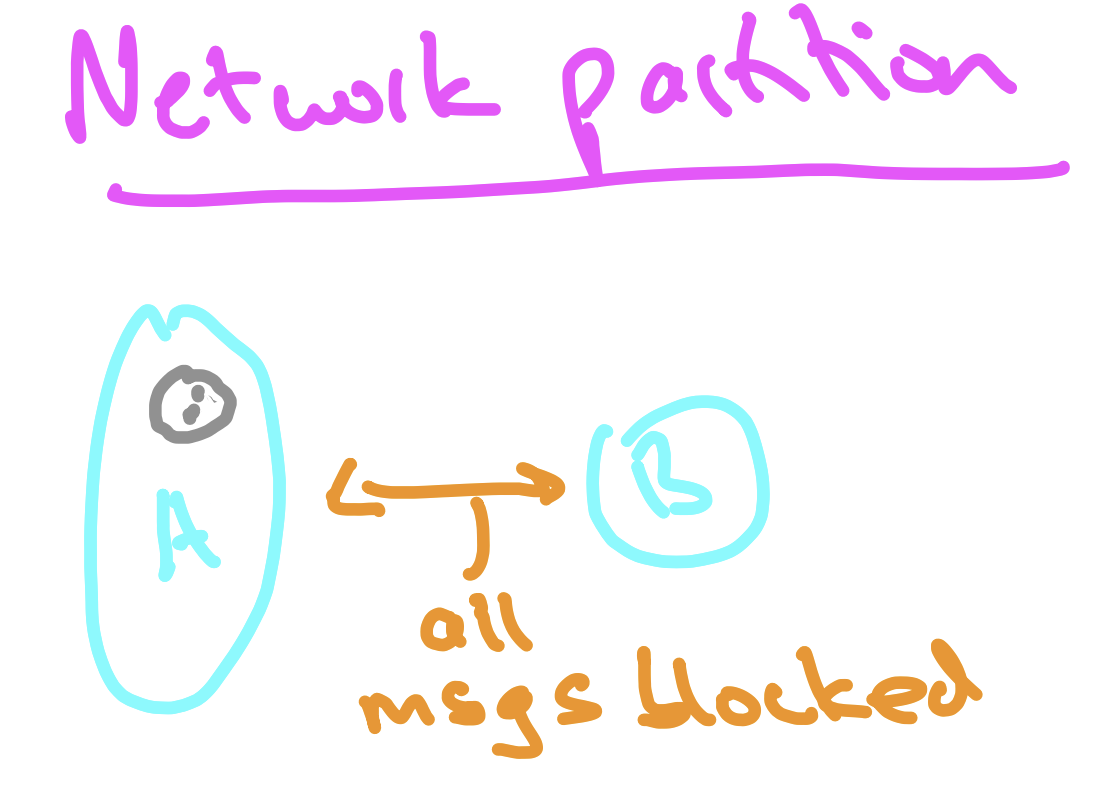
\includegraphics[scale = 0.5]{figures/f21.png}
    \caption{}
    \label{fig:mesh1}
\end{figure}\\
The CAP Principle states that no distributed system possess all three properties. In particular, if a system operates in a environment with network partitions (e.g., because it operates
over the Internet), it must give up on one on consistency or availability.\\

\textbf{The argument.} The reasoning behind the CAP Principle is pretty straightforward. Imagine a distributed system that is responsible for keeping track of (among other things) some variable $x$, and is suffering from a network partition as in Figure 6.2. For example, maybe
$x$ represents the number of times that the San Diego Padres have won the World Series
(currently, 0). Suppose the Padres win the ’22 Series and an excited fan issues a command
to the system to increment $x$ to 1, and suppose this command gets routed to a node $i$ in
the set A. Now consider an infinite stream of future queries about the value of $x$  that get
routed to node $i$. The node is in a catch-22 situation: if it ever answers “1,” it could cause
a violation of consistency (with all communication between A and B severed, nodes of B
would presumably answer “0” to the same query), but stubbornly answering “0” for the rest
of the time would violate availability.
A decision tree for design. This argument may strike you as a bit trivial (and to be
honest, it is), but it nonetheless suggests a useful decision tree to use when designing a
distributed system:
\begin{itemize}
    \item decide whether you want to worry about network partitions (e.g., because the system
will operate over the Internet) or not (e.g., because it will operate over a secure and
privately owned network);
    \item if not, demand both consistency and availability (somewhat analogous to our insistence
on both consistency and liveness for SMR protocols in the synchronous setting);
    \item if so, take a hard look at your application and decide which of consistency or availability
would be less painful to give up when there’s a network partition.

\end{itemize}
On the last point, you can imagine that different choices might make sense for different applications. For example, something like a bank might give up on availability while insisting
on consistency (e.g., the usual compromise made by traditional database systems)—having
its system go down for 24 hours while under attack is painful, but not as painful as the financial losses that could be caused by the exploitation of inconsistencies in account balances.
For something like a search engine, you can imagine prioritizing availability over consistency
(e.g., as offered by some NoSQL databases)—it’s not a big deal if two users in different parts
of the world see slightly different results for the same query, while downtime for a search
engine should be minimized at all costs.
Bringing the discussion back to blockchain protocol design, we’ll see an analogous dichotomy play out over the next two chapters: some SMR protocols (like Tendermint, see
chapter 7) give up on liveness when under attack (i.e., when in the asynchronous phase of
the partially synchronous model) while others (longest-chain consensus, see chapter 8) prefer
to give up on consistency.

\subsection{FLP Impossibility Theorem vs. CAP Principle}
The takeaways from the CAP Principle seem similar to those from the FLP impossibility
result (chapters 4 and 5): during a network attack (an asynchronous phase or a network
partition), you’re forced to choose between safety/consistency and liveness/availability.
Oddly, you almost never see the FLP impossibility result and the CAP Principle taught
in the same course—the former shows up in theory of distributed computing courses, the
latter in courses about distributed system design. But any blockchain expert should be aware
of both as well as the differences between them:
\begin{enumerate}
    \item The proof of the FLP impossibility result is hard. The argument behind the CAP
Principle is not. (I say this without judgment. As you've seen, these are the facts on
the ground.)
    \item Why is the argument for the CAP Principle so much easier? Because the setup allows
for messages (between the two sides of the partition) to be delayed forever (or simply
dropped)—there’s no requirement of eventual delivery, let alone a global stabilization
time. This means the message delivery adversary is potentially much more powerful
in the CAP case, and this extra power makes impossibility easy to argue.
The FLP impossibility result shows that safety and liveness are impossible even if the
adversary controlling message delivery is forced to eventually deliver every message—
with the less powerful adversary, impossibility is much harder to prove. (If you remember the proof, you’ll remember that we had to work quite hard to state and prove the
second lemma, which is the one that ensured the satisfaction of this constraint while
also extending the length of an ambiguous sequence of configurations.)
    \item In principle, there’s a different dimension in which the adversary controlling message
delivery is more powerful in the FLP setting than the CAP setting: in the latter, this
adversary is restricted to network partitions, while in the asynchronous model, this
adversary can do whatever it wants (subject to the eventual delivery constraint). In
hindsight, it seems that network partitions are a canonical attack and already capture
much of the power of more general strategies for adversarial message delivery.
    \item The adversary controlling message delivery in the CAP setting is so powerful that no
other adversary is needed. That is, the argument remains valid even if all the noes
are honest $(f = 0)$! By contrast, the FLP impossibility result no longer holds for the
$f = 0$—at least one faulty node really is needed.
\end{enumerate}
On the last point, you might recall from chapters 4 and 5 that the the proof of the FLP
impossibility result can be tweaked so that the result holds even with a single crash fault
(the most benign type, with the faulty node honest up until some point at which it gets
unplugged forever). And a crash fault does resemble a special case of infinite message
delays—for example, if the machine crashed immediately before it was about to send out
a bunch of messages, the effect is the same as if those messages suffered infinite delays. In a sense, what the FLP impossibility result really shows is that even the threat of a single
crash fault is enough to trigger the same conclusion (under attack, choose between safety
and liveness) that you would get somewhat trivially with infinite message delays.
Coming up next in chapter 7 is a possibility result which proves the “if” direction of
Theorem 6.1: there is a consensus protocol that, provided less than a third of the nodes are
Byzantine, guarantees safety and eventual (post-GST) liveness in the partially synchronous
model. As a bonus, the specific protocol that we’ll discuss (Tendermint) powers several
major blockchain protocols.




